\documentclass[11pt]{article}
% Hiding package calls and definitions
% {
\usepackage[margin=1in]{geometry}
\usepackage[utf8]{inputenc}
\usepackage[english]{babel}

\usepackage{pslatex}

\usepackage[pdftex]{graphicx}
\usepackage{siunitx}
\usepackage{caption}

\usepackage{booktabs,array}
\usepackage{tikz}
\usetikzlibrary{matrix,calc}
\usetikzlibrary{decorations.pathreplacing,angles,quotes}
\usetikzlibrary{bayesnet}
\usetikzlibrary{shapes.geometric,fit}

\newlength{\tikzheight}
\newlength{\tikzwidth}

\usepackage{amsfonts,amsmath,amssymb}
\usepackage{listings}
\usepackage{multicol}
\usepackage{multirow}
\usepackage{xcolor}
\usepackage{multicol}
\usepackage{algorithm}
\usepackage{algpseudocode}
\usepackage{adjustbox,lipsum}

\definecolor{c1}{RGB}{39,64,139}
\definecolor{c2}{RGB}{30,144,255}
\definecolor{c3}{RGB}{255,165,0}
\definecolor{c4}{RGB}{205,205,0}
\definecolor{c5}{RGB}{139,139,0}

\newcommand{\secref}[1]{\S\,\ref{#1}}
\newcommand{\appref}[1]{Appendix~\ref{#1}}
\newcommand{\figref}[1]{Fig.~\ref{#1}}
\newcommand{\tabref}[1]{Tab.~\ref{#1}}

\newcommand{\abs}[1]{\ensuremath\left|#1\right|}

\newcommand{\ie}{\emph{i.e.}}
\newcommand{\eg}{\emph{e.g.}}
\newcommand{\etc}{\emph{etc.}}

%
% The following macro is used to generate the header.
%
\newcommand{\lecture}[4]{
   \pagestyle{myheadings}
   \thispagestyle{plain}
   \noindent
   \begin{center}
   \framebox{
      \vbox{\vspace{1mm}
    \hbox to 6.58in {Technology and AI Learning Seminar (TAILS) \hfill Montana State University} 
    \hbox to 6.58in {Spring 2023 \hfill Dept. of Mathematics Sciences}
       \vspace{4mm}
       \hbox to 6.28in {\large\bf\hfill Lecture #1: #2  \hfill}
       \vspace{4mm}
       \hbox to 6.28in {\footnotesize Lecturer: #3 \hfill Scribe: #4}
      \vspace{1mm}}
   }
   \end{center}
   \markboth{Lecture #1: #2}{Lecture #1: #2}
   \vspace*{4mm}
}

\renewcommand{\vec}[1]{\ensuremath\bold{#1}}
%}

\begin{document}


\lecture{3}{Convolution}{Dominique Zosso, 2023-02-17}{Matt Pritting, Nick Boyer}
\tableofcontents
\null\hrule

\section*{Preamble}
    Repeat pictures and average. Noise drops out in the average but the signal stays the same (its how we found the higgs bozon). Note: doesn't work with sound. 	
    We can have a moving filter that does does an average over every point in space. 
    There is an underlying true signal affected by noise.  Noise is independent additive and white. 
    $$f[k] = u[k] + \eta [k]$$
    where $\eta ~ N(O,\sigma^2)$. $u[k]$ is underlying signal.




\section{Convolution}
    \textbf{Convolution of Two signals}
    $f,g:\mathbb{R}\to\mathbb{R}$ 
    $$(f*g)(t):=\int_{\mathbb{R}}f(\cdot)g(t-\cdot)d\cdot$$
    $$(f*g) [ k]:= \sum_{\cdot\in\mathbb{R}}f[ \cdot]g[k-\cdot]$$

     We are evaluating the similarity between $f$ and the flipped and shifted version of $g$. 
     If we get zero then the covariance is zero and there is no relation between the signals.
     See Figures 1-4 for a visual example of convolution.

    %Please feel free to reformat the figures -Matt :)
    \begin{figure}
        \begin{minipage}[t]{.49\textwidth}    
        \centering
        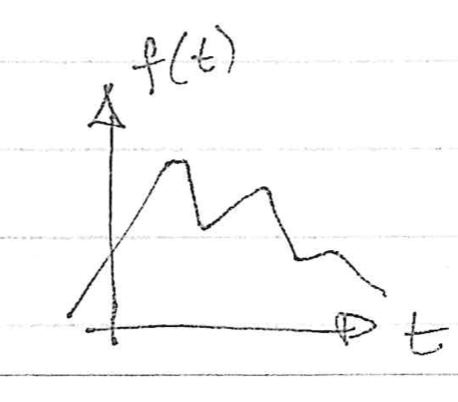
\includegraphics[width=\textwidth]{figures/lecture03/ffunction.png}
            \caption{One example function, f(t)}
        \label{fig:example function f(t)}
        \end{minipage}\hfill
        \begin{minipage}[t]{.49\textwidth}    
        \centering
        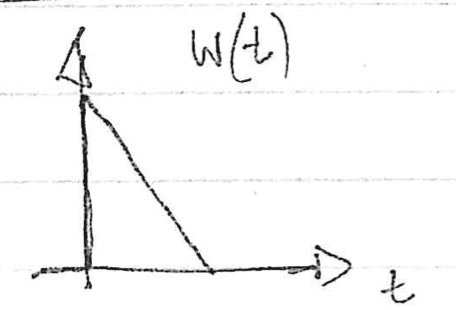
\includegraphics[width=\textwidth]{figures/lecture03/wfunction.png}
        \caption{A second example function w(t)}
        \label{fig:example function w(t)}
        \end{minipage}
    \end{figure}
    
    \begin{figure}
        \begin{minipage}[t]{.49\textwidth}    
        \centering
        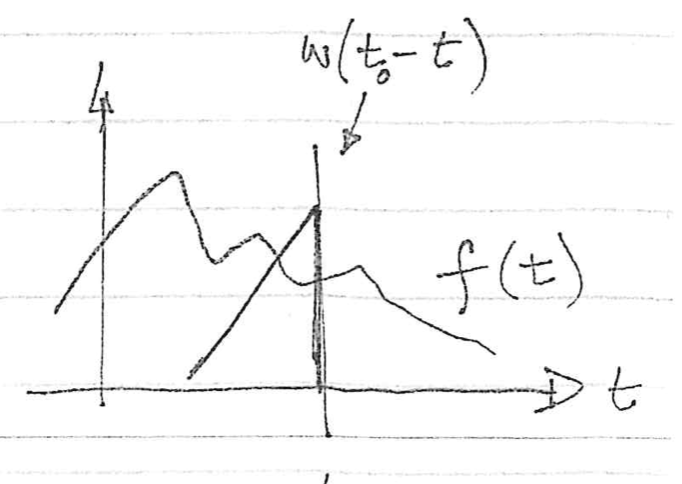
\includegraphics[width=\textwidth]{figures/lecture03/wt.png}
            \caption{Both f(t) and w($t_0$ - t) plotted}
        \label{fig:f(t) and w($t_0$ - t)}
        \end{minipage}\hfill
        \begin{minipage}[t]{.49\textwidth}    
        \centering
        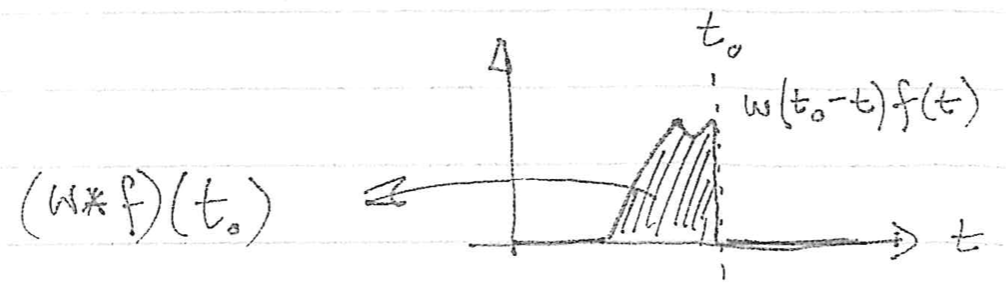
\includegraphics[width=\textwidth]{figures/lecture03/tconvw.png}
        \caption{The convolution of f(t) and w($t_0$ - t)}
        \label{fig:convolution of f(t) and w($t_0$ - t)}
        \end{minipage}
    \end{figure}

\subsection{Properties}
    \begin{enumerate}
        \item Commutative: $(f*g) = (g*f)$ 
        \item Associativity: $f*(g*h) = (f*g)*h$ 
        \item Distributive: $f*(g+h) = f*g+f*h$ 
        \item $(af)*g = a(f*g), a \in \mathbb{R}$
    \end{enumerate}
	
    So the convolution is a linear function. \\
    $$f*\delta = f$$
    $$\frac{d}{dt}(f*g) = \frac{df}{dt}*g = f*\frac{dg}{dt}$$

\subsection{Example of Convolution}
    Polynomial multiplication
    \begin{equation*}
        \begin{split}
            &(z^3+2z^2+1)(z+3)\\
            =&z^4 + 5z^3 + 6z^2 + z + 3\\ \\
                 &\hspace{2em} f(z) \cdot g(z) = [1 \hspace{0.5em} 2 \hspace{0.5em} 0 \hspace{0.5em} 1] \cdot [1 \hspace{0.5em} 3] \\
            &(f*g)[0] = \sum f[\cdot]g[0-\cdot] = f[]g[] \implies 3\\
            &(f*g)[1] = \sum f[\cdot]g[1-\cdot] = f[]g[] \implies 1\\
            &(f*g)[2] = \sum f[\cdot]g[2-\cdot] = f[]g[] \implies 6			
        \end{split}
    \end{equation*}
 
\subsection{Finite differences}

    $$f'[k] = \frac{f[k+1] - f[k]}{\Delta}= f*[1\,-1]$$ where $[1\,-1] \implies g[0]=-1/\Delta, g[-1] = 1/\Delta$
    $$f''[k] = \frac{f[k-1]-2f[k]+f[k+1]}{\Delta^2}= f*[1\,-2\,1]$$
    \begin{itemize}
    \item If $(f*g)[k] \gg 0$,
	then $f$ locally looks like $g^s$ at $k$\\
    \item If $ (f*g) \approx 0$,  
	then $f$ and $g^s$ are locally independent
	$f\perp g^s$ \\
    \item If $(f*g)[k] \ll 0$,
	then $f$ locally looks like additive inverse of $g^s$ at $k$\\
 \end{itemize}
 
\subsection{Convolution theorem}
    $$(f*g)(t) \iff F(\nu)\cdot G(\nu)$$
    $$(f\cdot g)(t) \iff F(\nu)* G(\nu)$$
    
    \subsubsection{Proof}
        \begin{equation*}
            \begin{split}
                \mathcal{F}[(f*g)](\nu) &= \int_{\mathbb{R}} (f*g)(t)e^{-j 2 \pi \nu t}dt \\
                &= \int_{\mathbb{R}} \int_{\mathbb{R}} f(\tau)g(t-\tau)(t)e^{-j 2 \pi \nu t}d\tau dt \\
                &= \int_{\mathbb{R}}f(\tau)[\int_{\mathbb{R}}g(t-\tau)e^{-j 2 \pi \nu t}dt]d\tau \\
                let \hspace{.3em} t' = t - \tau: \\
                &= \int_{\mathbb{R}}f(\tau)[\int_{\mathbb{R}}g(t')e^{-j 2 \pi \nu (t'+\tau)}dt']d\tau \\
                &= \int_{\mathbb{R}}f(\tau)e^{-j 2 \pi \nu \tau}d\tau 
                    \int_{\mathbb{R}}g(t')e^{-j 2 \pi \nu t'}dt'  \\
                &= F(\nu)G(\nu) \hspace{1em} \square
            \end{split}
        \end{equation*}

\subsection{Sampling}
    \begin{equation*}
        \begin{split}
            s_{\Delta}(t) &= \sum_{k\in\mathbb{Z}}\delta(t-k\Delta) \\
            &= \frac{1}{\Delta}\sum_{k\in\mathbb{Z}}e^{j 2 \pi \frac{kt}{\Delta}} \\ \\
            \mathcal{F}[s_{\Delta}(t)] &= S_{\Delta}[\nu] = \frac{1}{\Delta} \sum_{k\in\mathbb{Z}}\delta(v-\frac{k}{\Delta})
        \end{split}
    \end{equation*}
	
    \begin{equation*}
        \begin{split}
            \widetilde{f}(t) =& f(t)\cdot s_{\Delta}(t) \\ \\
            \widetilde{F}(t) =& F(t)*S_{\Delta}(t)\\
            =& \int_\mathbb{R} F(\cdot) S_{\Delta}(\nu-\cdot) d\cdot \\
            =& \frac{1}{\Delta} \int_\mathbb{R} F(\cdot) \sum_{k\in\mathbb{Z}} \delta(\nu-\cdot-\frac{k}{\Delta}) d\cdot \\
            =& \frac{1}{\Delta}\sum_{k\in\mathbb{Z}}\int_\mathbb{R}F(\cdot)\delta(u - \cdot-\frac{k}{\Delta})d\cdot \\
            =& \sum_{k\in\mathbb{Z}}F(v-\frac{k}{\Delta})
        \end{split}
    \end{equation*}

    We will only be able to recover F from $\widetilde{F}$ if $\frac{1}{\Delta} \geq 2\nu_{max}$ so that there is no overlap between signals in $\widetilde{F}$. See Figures 5-7 for an example. The left side of the convolution has an overlap in the signal which would not be recoverable. The right side however was sampled so that the original signal can be recovered.

    \begin{figure}
        \begin{minipage}[t]{.49\textwidth}    
        \centering
        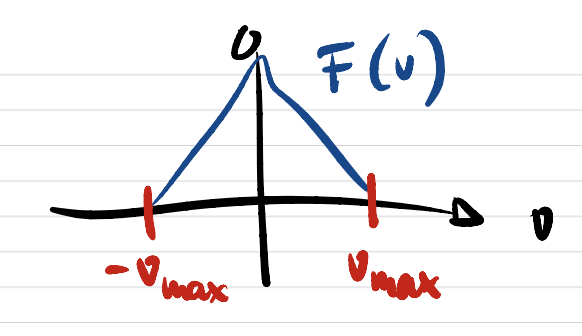
\includegraphics[width=\textwidth]{figures/lecture03/Fnu.png}
        \caption{A signal function F($\nu$})
        \label{fig:Signal Function f(nu)}
        \end{minipage}\hfill
        \begin{minipage}[t]{.49\textwidth}    
        \centering
        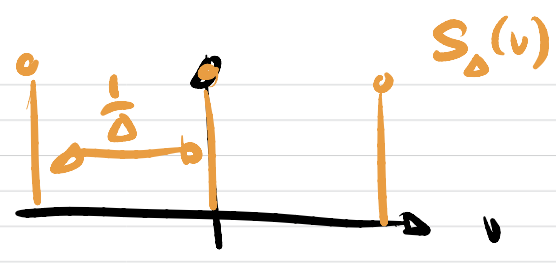
\includegraphics[width=\textwidth]{figures/lecture03/Sd.png}
        \caption{The sampling frequency $S_{\Delta}$}
        \label{fig:sampling frequency S_delta}
        \end{minipage}
    \end{figure}

    \begin{figure}
        \centering
        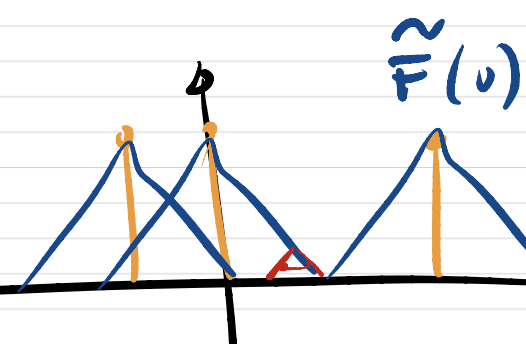
\includegraphics{figures/lecture03/FSd.png}
        \caption{$F(\nu)*S_\Delta(\nu)$}
        \label{fig:Convolution of F and S_delta}
    \end{figure}

\end{document}